%=========================================================
% MODULE 1 : INTRODUCTION TO MLOps
% Textbook 1: Part I (Chapters 1, 2, 3)
% Mark Treveil et al., Introducing MLOps, O'Reilly, 2020
%=========================================================

%=========================================================
\section{Module 1: Why Now and Challenges}
%=========================================================

\begin{frame}{Introduction to MLOps}
\begin{block}{Machine Learning Operations (MLOps)}
A process that helps organizations and business leaders generate long-term value and reduce the risk associated with data science, machine learning, and AI initiatives.
\end{block}
\vspace{0.2cm}
\begin{enumerate}
\item<1-> MLOps is quickly becoming a \textbf{critical component} of successful data science project deployment in the enterprise.
\item<2-> It is a \textbf{relatively new concept}, yet it has seemingly skyrocketed into the data science lexicon overnight.
\item<3-> This chapter covers:
    \begin{itemize}
    \item What MLOps is at a high level and its challenges.
    \item Why it is essential to a successful data science strategy.
    \item Why it is coming to the forefront \textbf{now}.
    \end{itemize}
\end{enumerate}
\end{frame}

%---------------------------------------------------------
\begin{frame}{MLOps Versus ModelOps Versus AIOps}
\begin{enumerate}
\item<1-> \textbf{MLOps / ModelOps:} A new discipline that emerged under these names in late 2018 and 2019; the two terms are largely used \textbf{interchangeably}.
\item<2-> Some argue \textbf{ModelOps is more general} than MLOps, since it covers any kind of model (e.g., rule-based models), not only machine learning models.
\item<3-> This course focuses on the \textbf{machine learning model life cycle}, hence the term \textbf{``MLOps''}.
\item<4-> \textbf{AIOps} is an entirely different topic: solving operational challenges \textbf{using AI} (i.e., AI for DevOps).
\item<5-> \textbf{AIOps example:} Predictive maintenance for network failures, alerting DevOps teams to possible problems before they arise.
\end{enumerate}
\end{frame}

%---------------------------------------------------------
\begin{frame}{Growth of MLOps}
\begin{columns}[T]
\begin{column}{0.52\textwidth}
\begin{figure}
\centering
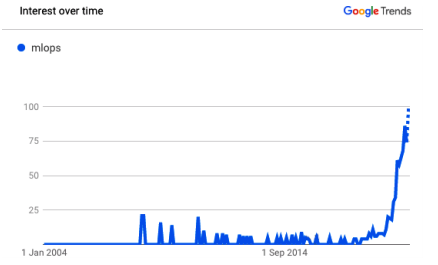
\includegraphics[width=\linewidth]{images/Fig1_1_mlops_growth.png}
\caption{Representation of the exponential growth of MLOps (not the parallel growth of the term ``ModelOps'')}
\end{figure}
\end{column}
\begin{column}{0.46\textwidth}
\begin{enumerate}\small
\item<1-> The chart shows Google Trends \textbf{interest over time} for the term ``mlops'' from 2004 onwards.
\item<2-> For more than a decade the interest remained \textbf{close to zero}, with only occasional spikes.
\item<3-> From around \textbf{2018--2019} the curve rises \textbf{exponentially}, reaching its peak (100).
\item<4-> This confirms MLOps as a \textbf{new and rapidly adopted} discipline in enterprise data science.
\end{enumerate}
\end{column}
\end{columns}
\end{frame}

%=========================================================
\subsection{Defining MLOps and Its Challenges}
%=========================================================

\begin{frame}{Defining MLOps}
\begin{block}{Definition}
At its core, MLOps is the \textbf{standardization and streamlining of machine learning life cycle management}.
\end{block}
\vspace{0.2cm}
\begin{enumerate}
\item<1-> From business problem to ML model, the steps at a very high level \textbf{seem straightforward}.
\item<2-> For most traditional organizations, developing \textbf{multiple ML models} and deploying them in production is \textbf{relatively new}.
\item<3-> Earlier, the number of models was manageable at a small scale, and there was less interest in understanding models and their dependencies company-wide.
\item<4-> With \textbf{decision automation} (decisions made without human intervention), models become more critical and \textbf{managing model risk} becomes a top-level concern.
\end{enumerate}
\end{frame}

%---------------------------------------------------------
\begin{frame}{Simple Machine Learning Model Life Cycle}
\begin{columns}[T]
\begin{column}{0.48\textwidth}
\begin{figure}
\centering
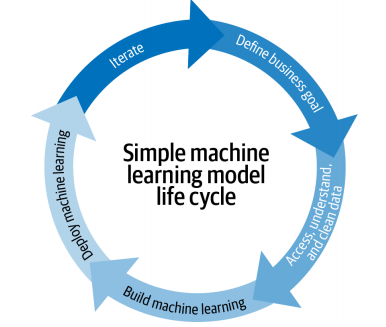
\includegraphics[width=\linewidth]{images/Fig1_2_simple_lifecycle.png}
\caption{A simple representation of the ML model life cycle, which often underplays the need for MLOps}
\end{figure}
\end{column}
\begin{column}{0.50\textwidth}
\begin{enumerate}\small
\item<1-> \textbf{Define business goal:} Identify the business problem the model must solve.
\item<2-> \textbf{Access, understand, and clean data:} Gather and prepare the data required.
\item<3-> \textbf{Build machine learning:} Train the ML model on the prepared data.
\item<4-> \textbf{Deploy machine learning:} Push the trained model into use.
\item<5-> \textbf{Iterate:} Repeat the cycle to improve the model.
\item<6-> This view \textbf{underplays} the real complexity of needs and tooling in an enterprise (see next figure).
\end{enumerate}
\end{column}
\end{columns}
\end{frame}

%---------------------------------------------------------
\begin{frame}{Challenges: Managing ML Life Cycles at Scale}
\begin{enumerate}
\item<1-> \textbf{There are many dependencies:}
    \begin{itemize}
    \item Data is constantly changing, and business needs shift as well.
    \item Results must be continually relayed back to the business to ensure the model in production meets the original goal.
    \end{itemize}
\item<2-> \textbf{Not everyone speaks the same language:}
    \begin{itemize}
    \item Business, data science, and IT teams are involved, but they do not use the same tools or share the same fundamental skills.
    \end{itemize}
\item<3-> \textbf{Data scientists are not software engineers:}
    \begin{itemize}
    \item They specialize in model building and assessment, not in writing applications.
    \item They juggle many roles; with staff turnover, they must manage models \textbf{they did not create}.
    \end{itemize}
\end{enumerate}
\end{frame}

%---------------------------------------------------------
\begin{frame}{Realistic Machine Learning Model Life Cycle}
\begin{columns}[T]
\begin{column}{0.42\textwidth}
\begin{figure}
\centering
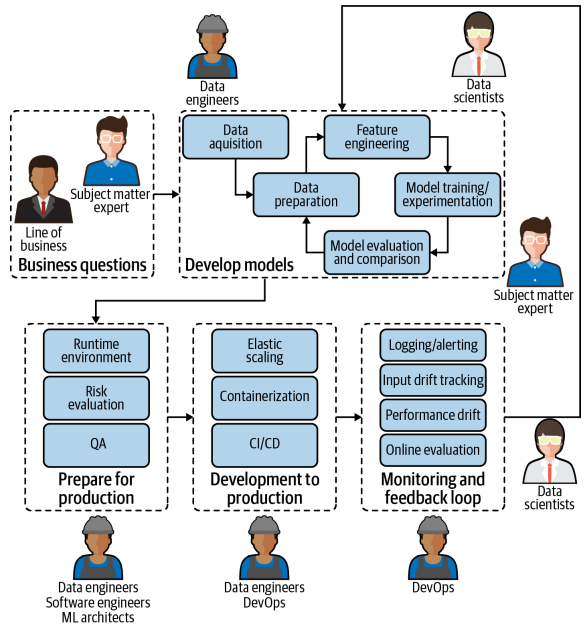
\includegraphics[height=0.64\textheight]{images/Fig1_3_realistic_lifecycle.png}
\caption{\scriptsize The realistic picture of an ML model life cycle inside an average organization today}
\end{figure}
\end{column}
\begin{column}{0.56\textwidth}
\begin{enumerate}\footnotesize
\item<1-> \textbf{Business questions:} Line of business and subject matter experts define the problem.
\item<2-> \textbf{Develop models:} Data acquisition $\rightarrow$ data preparation $\rightarrow$ feature engineering $\rightarrow$ model training/experimentation $\rightarrow$ model evaluation and comparison (data engineers, data scientists).
\item<3-> \textbf{Prepare for production:} Runtime environment, risk evaluation, QA (data engineers, software engineers, ML architects).
\item<4-> \textbf{Development to production:} Elastic scaling, containerization, CI/CD (data engineers, DevOps).
\item<5-> \textbf{Monitoring and feedback loop:} Logging/alerting, input drift tracking, performance drift, online evaluation (DevOps).
\item<6-> Feedback flows back to data scientists and SMEs; many people with \textbf{different skill sets and tools} are involved.
\end{enumerate}
\end{column}
\end{columns}
\end{frame}

%---------------------------------------------------------
\begin{frame}{MLOps and DevOps}
\begin{enumerate}
\item<1-> MLOps pulls heavily from \textbf{DevOps}, which streamlines the practice of software changes and updates.
\item<2-> Both center around:
    \begin{itemize}
    \item Robust automation and trust between teams.
    \item Collaboration and increased communication between teams.
    \item The end-to-end service life cycle (build, test, release).
    \item Prioritizing continuous delivery and high quality.
    \end{itemize}
\item<3-> \textbf{Critical difference:} Deploying software code is fundamentally different from deploying ML models.
\item<4-> Software code is \textbf{relatively static}, whereas data is \textbf{always changing}; models must constantly learn and adapt to new inputs.
\item<5-> ML models are made up of \textbf{both code and data}, which makes MLOps a new and unique discipline.
\end{enumerate}
\end{frame}

%---------------------------------------------------------
\begin{frame}{What About DataOps?}
\begin{enumerate}
\item<1-> \textbf{DataOps} was introduced in 2014 by IBM.
\item<2-> It seeks to provide \textbf{business-ready data} quickly, with focus on \textbf{data quality} and \textbf{metadata management}.
\item<3-> \textbf{Example:} If data a model relies on changes suddenly, DataOps alerts the business team and notifies the data team to investigate or revert a library upgrade and rebuild the partition.
\item<4-> MLOps \textbf{intersects} with DataOps, but goes further with additional key features (Chapter 3).
\item<5-> Until recently, teams could manage without centralized processes because they were not deploying ML models at scale.
\item<6-> Now, teams seek to formalize a \textbf{multi-stage, multi-discipline, multi-phase} process with a framework of MLOps best practices.
\end{enumerate}
\end{frame}

%=========================================================
\subsection{MLOps to Mitigate Risk}
%=========================================================

\begin{frame}{MLOps to Mitigate Risk}
\begin{enumerate}
\item<1-> MLOps is important to any team that has \textbf{even one model} in production.
\item<2-> Depending on the model, \textbf{continuous performance monitoring and adjusting} is essential.
\item<3-> By allowing safe and reliable operations, MLOps is key to \textbf{mitigating the risks} induced by ML models.
\item<4-> MLOps practices come at a \textbf{cost}; a proper \textbf{cost-benefit evaluation} should be performed for each use case.
\end{enumerate}
\end{frame}

%---------------------------------------------------------
\begin{frame}{Risk Assessment}
\begin{enumerate}
\item<1-> Risks vary widely: a monthly marketing recommendation engine is far lower stakes than a travel site whose \textbf{pricing and revenue} depend on an ML model.
\item<2-> A risk analysis should cover the risk that:
    \begin{itemize}
    \item The model is \textbf{unavailable} for a given period of time.
    \item The model returns a \textbf{bad prediction} for a given sample.
    \item Model \textbf{accuracy or fairness decreases} over time.
    \item The \textbf{skills} needed to maintain the model (data science talent) are lost.
    \end{itemize}
\item<3-> Risks are usually larger for models \textbf{deployed widely} and used outside the organization.
\item<4-> Risk assessment should be done at the \textbf{beginning} of each project and \textbf{reassessed periodically}.
\end{enumerate}
\end{frame}

%---------------------------------------------------------
\begin{frame}{Quantitative Risk Analysis: 5 $\times$ 5 Risk Matrix}
\begin{columns}[T]
\begin{column}{0.52\textwidth}
\begin{figure}
\centering
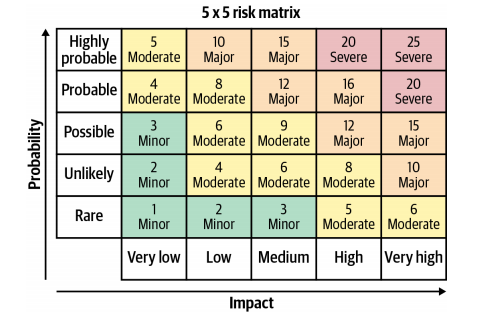
\includegraphics[width=\linewidth]{images/Fig1_4_risk_matrix.png}
\caption{A table that helps decision makers with quantitative risk analysis}
\end{figure}
\end{column}
\begin{column}{0.46\textwidth}
\begin{enumerate}\small
\item<1-> Risk is assessed on two metrics: \textbf{probability} (Rare $\rightarrow$ Highly probable) and \textbf{impact} (Very low $\rightarrow$ Very high).
\item<2-> Each is scored 1--5; their \textbf{product} gives the model's \textbf{severity} (1--25).
\item<3-> Severity is graded as \textbf{Minor}, \textbf{Moderate}, \textbf{Major}, or \textbf{Severe}.
\item<4-> Example: Possible (3) $\times$ High (4) = 12 $\rightarrow$ Major.
\item<5-> \textbf{Mitigation measures} are chosen based on this severity.
\end{enumerate}
\end{column}
\end{columns}
\end{frame}

%---------------------------------------------------------
\begin{frame}{Risk Mitigation}
\begin{enumerate}
\item<1-> MLOps becomes critical when a centralized team has \textbf{more than a handful} of operational models.
\item<2-> Without standardization, it is difficult to have a \textbf{global view} of the state of all models and take appropriate mitigation measures.
\item<3-> Full performance assessment is often only possible in the \textbf{production environment}.
\item<4-> Models are only as good as their training data; if production data changes, \textbf{performance may decrease rapidly}.
\item<5-> Model performance is sensitive to the \textbf{software environment} (versions of libraries such as scikit-learn, Python, or Linux) it runs in.
\item<6-> Deployment is \textbf{not the final step}; it is the beginning of monitoring the model and knowing how broadly it is used.
\end{enumerate}
\end{frame}

%---------------------------------------------------------
\begin{frame}{MLOps for Responsible AI}
\begin{enumerate}
\item<1-> \textbf{Intentionality:}
    \begin{itemize}
    \item Models are designed and behave in ways aligned with their purpose.
    \item Data comes from compliant and unbiased sources, with checks and balances on model bias.
    \item Includes \textbf{explainability}: results should be explainable by humans.
    \end{itemize}
\item<2-> \textbf{Accountability:}
    \begin{itemize}
    \item Centrally controlling, managing, and auditing the enterprise AI effort --- \textbf{no shadow IT}.
    \item Knowing which teams use what data, how, and in which models.
    \item Closely tied to \textbf{traceability}: where in the pipeline did something go wrong?
    \end{itemize}
\end{enumerate}
\end{frame}

%---------------------------------------------------------
\begin{frame}{Responsible AI and the Shift of Accountability}
\begin{enumerate}
\item<1-> ML models \textbf{lack the transparency} of traditional imperative code.
\item<2-> It is harder to understand which features determine a prediction, and to prove \textbf{regulatory compliance}.
\item<3-> Automation \textbf{shifts accountability} from the bottom of the hierarchy to the top.
\item<4-> Decisions once made by individuals (product price, loan approval) are now made by a model owned by a \textbf{data team manager or executive}.
\item<5-> Teams need good MLOps to practice Responsible AI, and Responsible AI \textbf{necessitates} MLOps strategies.
\end{enumerate}
\end{frame}

%=========================================================
\subsection{MLOps for Scale}
%=========================================================

\begin{frame}{MLOps for Scale}
\begin{enumerate}
\item<1-> MLOps is essential to \textbf{massively deploying} ML efforts and benefiting from economies of scale.
\item<2-> Going from a handful of models to \textbf{tens, hundreds, or thousands} requires MLOps discipline.
\item<3-> Good MLOps practices help teams, at a minimum, to:
    \begin{itemize}
    \item Keep track of \textbf{versioning}, especially with experiments in the design phase.
    \item Understand whether \textbf{retrained models are better} than previous versions, and promote better models to production.
    \item Ensure at defined periods (daily, monthly, etc.) that model performance is \textbf{not degrading} in production.
    \end{itemize}
\end{enumerate}
\end{frame}

%---------------------------------------------------------
\begin{frame}{Closing Thoughts}
\begin{enumerate}
\item<1-> MLOps practices are \textbf{not optional}; they are essential for scaling data science without putting the business at risk.
\item<2-> Without MLOps, teams face issues with \textbf{model quality and continuity}.
\item<3-> Worse, they may deploy models with real \textbf{negative business impact} (e.g., biased predictions).
\item<4-> Upper management should understand which models are in production and their business effect.
\item<5-> MLOps provides \textbf{transparency and accountability} down to the whole data pipeline (raw data to final output).
\end{enumerate}
\end{frame}

%=========================================================
\section{Module 1: People of MLOps}
%=========================================================

\begin{frame}{People of MLOps}
\begin{enumerate}
\item<1-> ML models are built primarily by data scientists, but MLOps involves \textbf{many roles} across the organization (see the realistic life cycle figure).
\item<2-> Each role has a different \textbf{skill set}, different \textbf{tools}, and a different \textbf{stake} in the model.
\item<3-> Key roles in MLOps:
    \begin{itemize}
    \item Subject Matter Experts (SMEs)
    \item Data Scientists and Data Engineers
    \item Software Engineers and DevOps
    \item Model Risk Manager / Auditor
    \item Machine Learning Architect
    \end{itemize}
\end{enumerate}
\end{frame}

%---------------------------------------------------------
\begin{frame}{Roles in MLOps and Their Responsibilities}
\small
\begin{table}
\centering
\renewcommand{\arraystretch}{1.25}
\scriptsize
\begin{tabular}{|p{3.2cm}|p{10cm}|}
\hline
\textbf{Role} & \textbf{Role in the ML Model Life Cycle} \\ \hline
Subject Matter Experts & Provide business questions, goals, and KPIs; evaluate whether model performance meets business needs. \\ \hline
Data Scientists & Build models that address the business question; deliver operationalizable models; assess model quality with SMEs. \\ \hline
Data Engineers & Optimize the retrieval and use of data to power ML models. \\ \hline
Software Engineers & Integrate ML models into the company's applications and systems. \\ \hline
DevOps & Build and test operational systems for security, performance, and availability; manage CI/CD pipelines. \\ \hline
Model Risk Manager/Auditor & Minimize overall risk from models in production; ensure compliance before deployment. \\ \hline
ML Architect & Ensure a scalable and flexible environment for ML pipelines from design to monitoring. \\ \hline
\end{tabular}
\end{table}
\end{frame}

%---------------------------------------------------------
\begin{frame}{Subject Matter Experts (SMEs)}
\begin{enumerate}
\item<1-> SMEs (line of business) \textbf{start the life cycle} by framing the business question.
\item<2-> They define \textbf{goals and KPIs} against which the model will ultimately be judged.
\item<3-> They bring \textbf{domain knowledge} needed during data exploration and feature engineering.
\item<4-> They evaluate whether model results are \textbf{useful for the business} and not just statistically good.
\item<5-> They take part in the \textbf{feedback loop}: monitoring results are relayed back to SMEs to confirm the model still meets the original goal.
\end{enumerate}
\end{frame}

%---------------------------------------------------------
\begin{frame}{Data Scientists and Data Engineers}
\begin{enumerate}
\item<1-> \textbf{Data Scientists:}
    \begin{itemize}
    \item Explore data, engineer features, train, evaluate, and compare models.
    \item Must deliver models that are \textbf{operationalizable}, reproducible, and explainable.
    \item Monitor model quality and drive retraining in the feedback loop.
    \end{itemize}
\item<2-> \textbf{Data Engineers:}
    \begin{itemize}
    \item Handle data acquisition and preparation pipelines.
    \item Ensure data is accessible, reliable, and available at the scale and speed required.
    \item Support preparing for production and deployment.
    \end{itemize}
\end{enumerate}
\end{frame}

%---------------------------------------------------------
\begin{frame}{Software Engineers and DevOps}
\begin{enumerate}
\item<1-> \textbf{Software Engineers:}
    \begin{itemize}
    \item Integrate ML models into applications and business systems.
    \item Ensure models work seamlessly with non-ML components.
    \end{itemize}
\item<2-> \textbf{DevOps:}
    \begin{itemize}
    \item Build and operate production systems: runtime, containerization, elastic scaling.
    \item Own \textbf{CI/CD pipelines} for automated testing and deployment.
    \item Monitor resource usage, latency, logging, and alerting in production.
    \end{itemize}
\end{enumerate}
\end{frame}

%---------------------------------------------------------
\begin{frame}{Model Risk Manager/Auditor and ML Architect}
\begin{enumerate}
\item<1-> \textbf{Model Risk Manager / Auditor:}
    \begin{itemize}
    \item Minimizes the overall risk to the company from models in production.
    \item Ensures compliance with internal and external (regulatory) requirements.
    \item Reviews documentation, validation, and sign-offs before deployment.
    \end{itemize}
\item<2-> \textbf{Machine Learning Architect:}
    \begin{itemize}
    \item Designs a scalable and flexible environment for ML pipelines.
    \item Selects and introduces technologies that improve performance in production.
    \item Bridges data science, data engineering, and IT infrastructure.
    \end{itemize}
\end{enumerate}
\end{frame}

%=========================================================
\section{Module 1: Key MLOps Features}
%=========================================================

\begin{frame}{Key MLOps Features}
\begin{enumerate}
\item<1-> MLOps affects many roles and many parts of the ML life cycle.
\item<2-> The \textbf{five key components} of MLOps are:
    \begin{enumerate}
    \item Development
    \item Deployment
    \item Monitoring
    \item Iteration
    \item Governance
    \end{enumerate}
\item<3-> These are introduced here at a high level and form the foundation for Chapters 4--8.
\end{enumerate}
\end{frame}

%=========================================================
\subsection{A Primer on Machine Learning}
%=========================================================

\begin{frame}{A Primer on Machine Learning}
\begin{block}{Machine Learning}
The science of computer algorithms that automatically \textbf{learn and improve from experience} rather than being explicitly programmed.
\end{block}
\vspace{0.1cm}
\begin{enumerate}
\item<1-> Algorithm selection has a \textbf{direct impact} on MLOps processes.
\item<2-> Algorithms analyze sample data (\textbf{training data}) to build a model that makes predictions.
\item<3-> \textbf{Examples:} Identifying an electricity meter type from a photo; recommending insurance products based on behavior of similar customers.
\item<4-> On \textbf{unseen data}, the model predicts assuming it is related to the previous data.
\item<5-> Models range from simple \textbf{decision trees} and \textbf{logistic regression} to complex \textbf{deep learning} models.
\end{enumerate}
\end{frame}

%=========================================================
\subsection{Model Development}
%=========================================================

\begin{frame}{Model Development: Establishing Business Objectives}
\begin{enumerate}
\item<1-> Development starts with a \textbf{business objective}, e.g., reducing fraudulent transactions to $<$ 0.1\% or identifying faces in social media photos.
\item<2-> Objectives come with performance targets, infrastructure requirements, and cost constraints, captured as \textbf{KPIs}.
\item<3-> KPIs enable the business performance of models in production to be \textbf{monitored}.
\item<4-> ML projects are part of a larger project that impacts technologies, processes, and people, so objectives include \textbf{change management}.
\item<5-> The required degree of \textbf{transparency} strongly influences the choice of algorithm and the need to explain predictions.
\end{enumerate}
\end{frame}

%---------------------------------------------------------
\begin{frame}{Data Sources and Exploratory Data Analysis}
\small
\begin{enumerate}
\item<1-> SMEs and data scientists begin by searching for suitable input data --- often the \textbf{most arduous} part of the journey.
\item<2-> \textbf{Key questions for finding data:}
    \begin{itemize}
    \item What relevant datasets are available? Are they accurate and reliable?
    \item How can stakeholders access the data? What \textbf{features} can be made by combining sources?
    \item Will the data be available in real time?
    \item Is labeling with ``ground truth'' needed, or does unsupervised learning make sense? At what cost?
    \end{itemize}
\item<3-> \textbf{More questions:}
    \begin{itemize}
    \item What platform should be used? How will data be updated after deployment?
    \item Will the model's use reduce the \textbf{representativeness} of the data?
    \item How will the KPIs be measured?
    \end{itemize}
\end{enumerate}
\end{frame}

%---------------------------------------------------------
\begin{frame}{Data Governance Questions and EDA}
\begin{enumerate}
\item<1-> \textbf{Data governance constraints} raise more questions:
    \begin{itemize}
    \item Can the datasets be used for this purpose? What are the terms of use?
    \item Is there \textbf{PII} that must be redacted or anonymized?
    \item Are there features (e.g., gender) that legally cannot be used?
    \item Are minority populations represented well enough for equivalent performance?
    \end{itemize}
\item<2-> \textbf{Exploratory Data Analysis (EDA)} helps to:
    \begin{itemize}
    \item Build hypotheses about the data.
    \item Identify data cleaning requirements.
    \item Inform the selection of potentially significant features.
    \end{itemize}
\item<3-> EDA can be done \textbf{visually} for intuition or \textbf{statistically} for rigor.
\end{enumerate}
\end{frame}

%---------------------------------------------------------
\begin{frame}{Feature Engineering and Selection; Training and Evaluation}
\begin{enumerate}
\item<1-> \textbf{Feature engineering} transforms raw data into ``features'' that better represent the underlying problem.
\item<2-> Features are \textbf{arrays of numbers of fixed size} --- the only object ML algorithms understand.
\item<3-> It includes \textbf{data cleansing}, often the largest part of an ML project in time spent.
\item<4-> \textbf{Training} is iterative: test algorithms, generate features, adapt selections, tune hyperparameters; it is the most \textbf{compute-intensive} step.
\item<5-> An \textbf{experiment tracking tool} records data, features, parameters, and metrics so experiments can be compared side-by-side.
\item<6-> The best solution needs \textbf{quantitative} (accuracy, error) and \textbf{qualitative} (explainability, ease of deployment) criteria.
\end{enumerate}
\end{frame}

%---------------------------------------------------------
\begin{frame}{Reproducibility}
\begin{enumerate}
\item<1-> Many experiments are short-lived, but \textbf{significant versions} of a model must be saved.
\item<2-> \textbf{Reproducibility} aims to save enough about the environment so the model can be \textbf{reproduced with the same results from scratch}.
\item<3-> Without it, data scientists cannot confidently iterate on models.
\item<4-> Nor can they hand the model to \textbf{DevOps} to check that the lab result is faithfully reproduced in production.
\item<5-> True reproducibility requires \textbf{version control of all assets and parameters}, including training/evaluation data and the software environment.
\end{enumerate}
\end{frame}

%---------------------------------------------------------
\begin{frame}{Responsible AI in Model Development}
\begin{enumerate}
\item<1-> DevOps must understand how to \textbf{verify} the model: what it does, how to test it, expected results.
\item<2-> Regulated industries must document how the model was built and tuned; critical models may be \textbf{independently rebuilt}.
\item<3-> \textbf{Documentation} is the standard solution; automated model documentation helps, but some must be written by hand.
\item<4-> Standard performance measures do not explain \textbf{how} predictions are made.
\item<5-> The ``how'' is needed to sanity-check the model, improve features, and ensure \textbf{fairness} (sex, age, race) --- the field of \textbf{explainability}.
\end{enumerate}
\end{frame}

%---------------------------------------------------------
\begin{frame}{Explainability Techniques}
\begin{enumerate}
\item<1-> \textbf{Partial dependence plots:} Look at the marginal impact of features on the predicted outcome.
\item<2-> \textbf{Subpopulation analyses:} Look at how the model treats specific subpopulations; the basis of many fairness analyses.
\item<3-> \textbf{Individual model predictions (e.g., Shapley values):} Explain how each feature value contributes to a specific prediction.
\item<4-> \textbf{What-if analysis:} Helps the user understand the sensitivity of the prediction to its inputs.
\item<5-> MLOps work done up front in development makes models \textbf{easier to manage} later, especially in production.
\end{enumerate}
\end{frame}

%=========================================================
\subsection{Productionalization and Deployment}
%=========================================================

\begin{frame}{Productionalization and Deployment}
\begin{enumerate}
\item<1-> Presents an \textbf{entirely different} set of technical challenges than model development.
\item<2-> It is the domain of the \textbf{software engineer} and the \textbf{DevOps team}.
\item<3-> Information exchange between data scientists and these teams must not be underestimated.
\item<4-> Without effective collaboration, \textbf{delays or failures to deploy} are inevitable.
\end{enumerate}
\end{frame}

%---------------------------------------------------------
\begin{frame}{Model Deployment Types and Contents}
\begin{enumerate}
\item<1-> \textbf{Model-as-a-service (live-scoring model):} Deployed in a framework providing a \textbf{REST API endpoint} that responds to requests in real time.
\item<2-> \textbf{Embedded model:} Packaged into an application which is then published, e.g., an application providing \textbf{batch-scoring}.
\item<3-> A deployed model comprises \textbf{code} (Python, R, or Java) and \textbf{data artifacts}, with version dependencies on runtimes and packages.
\item<4-> Different versions in production \textbf{may cause predictions to differ}.
\item<5-> \textbf{Portable formats} (PMML, PFA, ONNX, POJO) reduce dependencies, but support limited algorithms and may behave subtly differently.
\end{enumerate}
\end{frame}

%---------------------------------------------------------
\begin{frame}{Containerization}
\begin{enumerate}
\item<1-> An increasingly popular solution to \textbf{dependency headaches} when deploying ML models.
\item<2-> Container technologies such as \textbf{Docker} are lightweight alternatives to virtual machines.
\item<3-> Applications run in \textbf{independent, self-contained environments} matching each model's exact requirements.
\item<4-> Enable new models to be seamlessly deployed using the \textbf{blue-green deployment} technique.
\item<5-> Compute can be \textbf{scaled elastically} using multiple containers.
\item<6-> Orchestration of many containers is handled by \textbf{Kubernetes}, in the cloud or on-premise.
\end{enumerate}
\end{frame}

%---------------------------------------------------------
\begin{frame}{Model Deployment Requirements}
\begin{enumerate}
\item<1-> \textbf{Rapid, automated deployment} is always preferred to labor-intensive processes.
\item<2-> For \textbf{short-lifetime, self-service} applications, a fully automated single-step push-to-production may be adequate (resources capped by Linux cgroups; simple UIs with Flask).
\item<3-> For \textbf{customer-facing, mission-critical} use cases, a robust \textbf{CI/CD pipeline} is required.
\item<4-> In heavily regulated industries (finance, pharmaceuticals), checks are extensive and may involve \textbf{manual intervention}.
\item<5-> MLOps, like DevOps, aims to \textbf{automate CI/CD} as far as possible: faster deployment, more regression testing, fewer errors.
\end{enumerate}
\end{frame}

%---------------------------------------------------------
\begin{frame}{Robust CI/CD Pipeline for Mission-Critical Models}
\begin{enumerate}
\item<1-> Ensuring all coding, documentation, and sign-off standards have been met.
\item<2-> Re-creating the model in something approaching the production environment.
\item<3-> Revalidating the model accuracy.
\item<4-> Performing explainability checks.
\item<5-> Ensuring all governance requirements have been met.
\item<6-> Checking the quality of any data artifacts.
\item<7-> Testing resource usage under load.
\item<8-> Embedding into a more complex application, including integration tests.
\end{enumerate}
\end{frame}

%=========================================================
\subsection{Monitoring}
%=========================================================

\begin{frame}{Monitoring}
\begin{enumerate}
\item<1-> After deployment, the model must \textbf{continue to perform well} over time.
\item<2-> Good performance means different things to \textbf{DevOps}, \textbf{data scientists}, and the \textbf{business}.
\item<3-> \textbf{DevOps concerns:}
    \begin{itemize}
    \item Is the model getting the job done \textbf{quickly enough}?
    \item Is it using a sensible amount of \textbf{memory and processing time}?
    \end{itemize}
\item<4-> This is traditional IT performance monitoring; ML resource demands are similar to traditional software.
\item<5-> Scalability matters, e.g., when \textbf{retraining in production}; deep learning needs more resources than decision trees.
\end{enumerate}
\end{frame}

%---------------------------------------------------------
\begin{frame}{Data Scientist Concerns}
\begin{enumerate}
\item<1-> ML models \textbf{degrade over time}, since they are models of the data they were trained on --- a problem not faced by traditional software.
\item<2-> The real world does not stand still:
    \begin{itemize}
    \item A fraud model trained six months ago will not reflect a \textbf{new type of fraud}.
    \item An ad model becomes less relevant if a website attracts a \textbf{younger user base}.
    \end{itemize}
\item<3-> When performance becomes unacceptable, \textbf{retraining} is necessary.
\item<4-> Retraining frequency depends on how fast the world changes, accuracy needed, and ease of building/deploying a better model.
\item<5-> Two approaches to detect degradation: \textbf{ground truth} and \textbf{input drift}.
\end{enumerate}
\end{frame}

%---------------------------------------------------------
\begin{frame}{Ground Truth and Input Drift}
\begin{enumerate}
\item<1-> \textbf{Ground truth:} The correct answer to the question the model was asked (e.g., ``Is this transaction actually fraudulent?'').
\item<2-> Sometimes obtained \textbf{rapidly} (ad clicks within seconds); often \textbf{slowly} (fraud reported up to a month later, or never).
\item<3-> Slow ground truth prevents accurate daily monitoring; if rapid feedback is needed, use input drift.
\item<4-> \textbf{Input drift:} If recent requests differ distinctly from training data, model performance is likely compromised.
\item<5-> All required data \textbf{already exists} --- no need to wait for ground truth.
\item<6-> Drift identification brings \textbf{agility} to enterprise AI efforts (detailed in Chapter 7).
\end{enumerate}
\end{frame}

%---------------------------------------------------------
\begin{frame}{Business Concerns}
\begin{enumerate}
\item<1-> The business takes a \textbf{holistic} view:
    \begin{itemize}
    \item Is the model delivering \textbf{value} to the enterprise?
    \item Do benefits outweigh the \textbf{cost} of developing and deploying it?
    \end{itemize}
\item<2-> The original \textbf{KPIs} should be monitored, automatically where possible --- rarely trivial.
\item<3-> Even monitoring fraud rate does not answer: what is the \textbf{net gain in dollars}?
\item<4-> In the absence of a ``dollar-o-meter,'' monitoring \textbf{business KPIs} is the best option.
\item<5-> Choose a \textbf{baseline} that isolates ML value, e.g., compare against a \textbf{rule-based} model built from subject matter expertise.
\end{enumerate}
\end{frame}

%=========================================================
\subsection{Iteration and Life Cycle}
%=========================================================

\begin{frame}{Iteration and Life Cycle}
\begin{enumerate}
\item<1-> Developing and deploying \textbf{improved versions} is essential and one of the more challenging parts of MLOps.
\item<2-> Reasons for a new version: \textbf{model drift}, refined business objectives/KPIs, or a \textbf{better model design}.
\item<3-> In fast-moving environments, daily retraining and redeployment are often \textbf{automated}.
\item<4-> Pitfalls even in simple retraining:
    \begin{itemize}
    \item Does the new training data look as expected? (automated validation)
    \item Is the data complete and consistent?
    \item Are feature distributions similar to the previous training set?
    \end{itemize}
\item<5-> Compare new and live model metrics on the \textbf{same dataset}; if variation is wide, seek \textbf{manual intervention}.
\end{enumerate}
\end{frame}

%---------------------------------------------------------
\begin{frame}{Retraining Scenarios}
\begin{enumerate}
\item<1-> Even ``simple'' retraining needs multiple datasets: scoring data reconciliation (with ground truth), cleaning/validation, the previous model, and checks.
\item<2-> Other scenarios are more complicated, making \textbf{automated redeployment unlikely}.
\item<3-> \textbf{Drift-motivated retraining:} If new labeled data exists, retraining with it has the best cost-benefit ratio.
\item<4-> If ground truth is slow, there may be \textbf{little new labeled data}.
\item<5-> Data scientists must understand the drift, \textbf{adjust existing training data}, and design mitigations (e.g., remove a feature, resample rows).
\item<6-> Time needed grows with the amount of \textbf{modeling debt}.
\end{enumerate}
\end{frame}

%---------------------------------------------------------
\begin{frame}{The Feedback Loop: Shadow Testing and A/B Testing}
\begin{enumerate}
\item<1-> The live scoring and retraining environments are usually \textbf{distinct}, so evaluation in retraining may be compromised.
\item<2-> \textbf{Shadow testing:} New version runs alongside the incumbent; the incumbent answers, the new version's results are only \textbf{logged}, then compared statistically.
\item<3-> Shadow scoring gives SMEs visibility on future versions for a \textbf{smoother transition}.
\item<4-> When outcomes depend on the user's reaction (ad clicks), \textbf{A/B testing} is more common.
\item<5-> \textbf{A/B testing:} Requests are \textbf{split} between the two models; each request is processed by only one model.
\end{enumerate}
\end{frame}

%---------------------------------------------------------
\begin{frame}{A/B Testing Variants}
\begin{enumerate}
\item<1-> Statistically meaningful A/B conclusions require \textbf{careful planning}.
\item<2-> \textbf{Fixed-horizon test:} Wait until a predetermined number of samples is tested; ``peeking'' early is \textbf{unreliable}.
\item<3-> In a live commercial environment, every bad prediction costs money, so not stopping early can be \textbf{expensive}.
\item<4-> \textbf{Bayesian / multi-armed bandit tests} aim to draw conclusions \textbf{more quickly}.
\item<5-> Multi-armed bandit testing is \textbf{adaptive}: traffic to underperforming models is reduced, lowering business cost.
\end{enumerate}
\end{frame}

%---------------------------------------------------------
\begin{frame}{Iterating on the Edge}
\begin{enumerate}
\item<1-> Iterating on models deployed to \textbf{millions of devices} (phones, sensors, cars) poses different challenges.
\item<2-> \textbf{Centralized training:} Relay feedback to a central point. Tesla's autopilot (500,000+ cars) retrains about 50 neural networks using 70,000 GPU hours.
\item<3-> \textbf{Federated learning:} Google's GBoard retrains locally on each phone and sends a summary of improvements, which are averaged into the shared model.
\item<4-> Benefits of federated learning:
    \begin{itemize}
    \item Personal data need not be collected centrally.
    \item Improved model is usable immediately on each phone.
    \item Overall power consumption goes down.
    \end{itemize}
\end{enumerate}
\end{frame}

%=========================================================
\subsection{Governance}
%=========================================================

\begin{frame}{Governance}
\begin{block}{Governance}
The set of controls placed on a business to ensure that it delivers on its responsibilities to all stakeholders --- shareholders, employees, the public, and national governments.
\end{block}
\vspace{0.1cm}
\begin{enumerate}
\item<1-> Responsibilities include \textbf{financial, legal, and ethical} obligations, all underpinned by \textbf{fairness}.
\item<2-> \textbf{Legal obligations} existed before ML: financial regulations protect against fraud; pharmaceutical rules safeguard public health.
\item<3-> Broader legislation protects vulnerable sectors and ensures a level playing field on sex, race, age, or religion.
\item<4-> Data regulations such as \textbf{GDPR (2016, EU)} and \textbf{CCPA (2018, California)} have had immense impact on ML.
\end{enumerate}
\end{frame}

%---------------------------------------------------------
\begin{frame}{GDPR Principles}
\begin{enumerate}
\item<1-> GDPR sets principles for \textbf{processing personal data} (collection, storage, alteration, use); CCPA closely mirrors them.
\item<2-> The principles are:
    \begin{itemize}
    \item Lawfulness, fairness, and transparency
    \item Purpose limitation
    \item Data minimization
    \item Accuracy
    \item Storage limitation
    \item Integrity and confidentiality (security)
    \item Accountability
    \end{itemize}
\item<3-> The \textbf{EU} is leading planned legislation defining acceptable uses of AI; businesses must heed yet more regulation.
\end{enumerate}
\end{frame}

%---------------------------------------------------------
\begin{frame}{Moral Responsibility and Governance Categories}
\begin{enumerate}
\item<1-> Businesses increasingly care about moral responsibility beyond legislation, as seen in \textbf{ESG} performance indicators.
\item<2-> \textbf{Trust} matters to consumers and shareholders; businesses engage with \textbf{Responsible AI}.
\item<3-> Governance in MLOps is challenging: complex processes, opaque technology, fundamental data dependence.
\item<4-> \textbf{Data governance:} A framework for ensuring appropriate use and management of data.
\item<5-> \textbf{Process governance:} Well-defined processes ensuring all governance considerations are addressed at the right point in the life cycle, with a full and accurate record.
\end{enumerate}
\end{frame}

%---------------------------------------------------------
\begin{frame}{Data Governance}
\begin{enumerate}
\item<1-> Addresses questions such as:
    \begin{itemize}
    \item What is the data's \textbf{provenance}? Under what terms was it collected?
    \item Is the data accurate and up to date?
    \item Is there \textbf{PII} or sensitive data that should not be used?
    \end{itemize}
\item<2-> Understanding \textbf{data lineage}, especially at feature level, is complex but essential for GDPR compliance.
\item<3-> Anonymizing or pseudo-anonymizing data is \textbf{not always sufficient}; individuals may still be singled out.
\item<4-> \textbf{Accidental bias:} A recruitment model discriminated against women by learning from all-female schools' underrepresentation in upper management (Amazon, 2018).
\end{enumerate}
\end{frame}

%---------------------------------------------------------
\begin{frame}{Data Lineage Tools}
\begin{enumerate}
\item<1-> Data governance tools are still \textbf{in their infancy}.
\item<2-> Most focus on two data lineage questions:
    \begin{itemize}
    \item Where did the information in this dataset \textbf{come from}, and how can I use it?
    \item How is this dataset \textbf{used}, and what are the downstream implications if I change it?
    \end{itemize}
\item<3-> Neither is easy to answer fully in real-world pipelines.
\item<4-> \textbf{Example:} If a Python function processes several datasets in memory to produce one output, from what information was each cell derived?
\end{enumerate}
\end{frame}

%---------------------------------------------------------
\begin{frame}{Process Governance}
\begin{enumerate}
\item<1-> Formalizes MLOps steps and associates actions: \textbf{reviews, sign-offs}, and capture of supporting materials.
\item<2-> \textbf{Aims:}
    \begin{itemize}
    \item Every governance consideration is made at the correct time (e.g., no deployment until validation passes).
    \item Enable \textbf{oversight} by auditors, risk managers, and compliance officers.
    \end{itemize}
\item<3-> \textbf{Why it is hard:}
    \begin{itemize}
    \item ML processes are rarely easy to define; understanding is spread across teams.
    \item Every team must adopt it wholeheartedly.
    \item Heavy-weight processes will be \textbf{subverted} by teams.
    \end{itemize}
\item<4-> Most common today in heavily regulated sectors such as \textbf{finance}.
\end{enumerate}
\end{frame}

%---------------------------------------------------------
\begin{frame}{Closing Thoughts}
\begin{enumerate}
\item<1-> MLOps features and processes \textbf{cannot be ignored} by data teams or the data-driven organization.
\item<2-> MLOps is \textbf{not a checklist item} (``yes, we do MLOps!'').
\item<3-> It is a complex interplay of \textbf{technologies, processes, and people}.
\item<4-> It requires \textbf{discipline and time} to do correctly.
\item<5-> The following chapters go deeper into each life cycle component, starting with \textbf{Developing Models} (Module 2).
\end{enumerate}
\end{frame}